From these three languages we can see the importance of parallelization and concurrency in different applications, as well as how greatly each vary. This can be from specific inspiration or reasoning to solve a problem, as Go and Clojure have a range of tools and larger forms of importing than Swift, which focuses on the implementations of other languages and applications.

Each also have their own way of dealing with lack of hardware or dealing with concurrency to the point where variable initialization is taken into account as to what default values will be read if nothing reaches to assign it. It has also been asked if the variable should be assigned before reading as well, creating interesting paradigms and designs for each language.

Their applications have wide variations, from scientific computing in clusters or grids to working with servers or local applications. This expanse in usage and features is what makes these languages not only verbose, but also fast, using concurrency to speed up their general performance.

\subsection{Comparison: Java vs. Go vs. Clojure}
    Earlier we described a programming problem that we gave each of our programs to solve, and later described how Swift isn't meant for this type of use and focuses more on optimizing different applications, leaving us Go and Clojure. We will be comparing these two with Java, using several different matrix sizes (NxN) as the input and seeing how it corresponds with its execution speed.

    In our Clojure and Go sections, we saw how the execution time output for each matrix size NxN. For our Java implementation using threads, we received our own set of results.
    \\~\\
    \begin{tabular}{ | l | l | l | p{5cm} |}
    \hline
    N & Average Number of Seconds to Completion \\ \hline
    100 & 0.08 \\ \hline
    250 & 0.28 \\ \hline
    500 & 11.3 \\ \hline
    750 & 25.5 \\ \hline
    1000 & 45.1 \\ \hline
    1500 & 101.6 \\ \hline
    2000 & 181.3 \\ \hline

    \hline
    \end{tabular}\\~\\

    Using our previous results as well as our Java results, we created a graph comparing each language implementation on the number of seconds need to complete the matrix multiplication to the size of the square matrix used. We found that Java, as expected, performed the worse in general while Clojure beat our Go implementation when using larger matricies.

    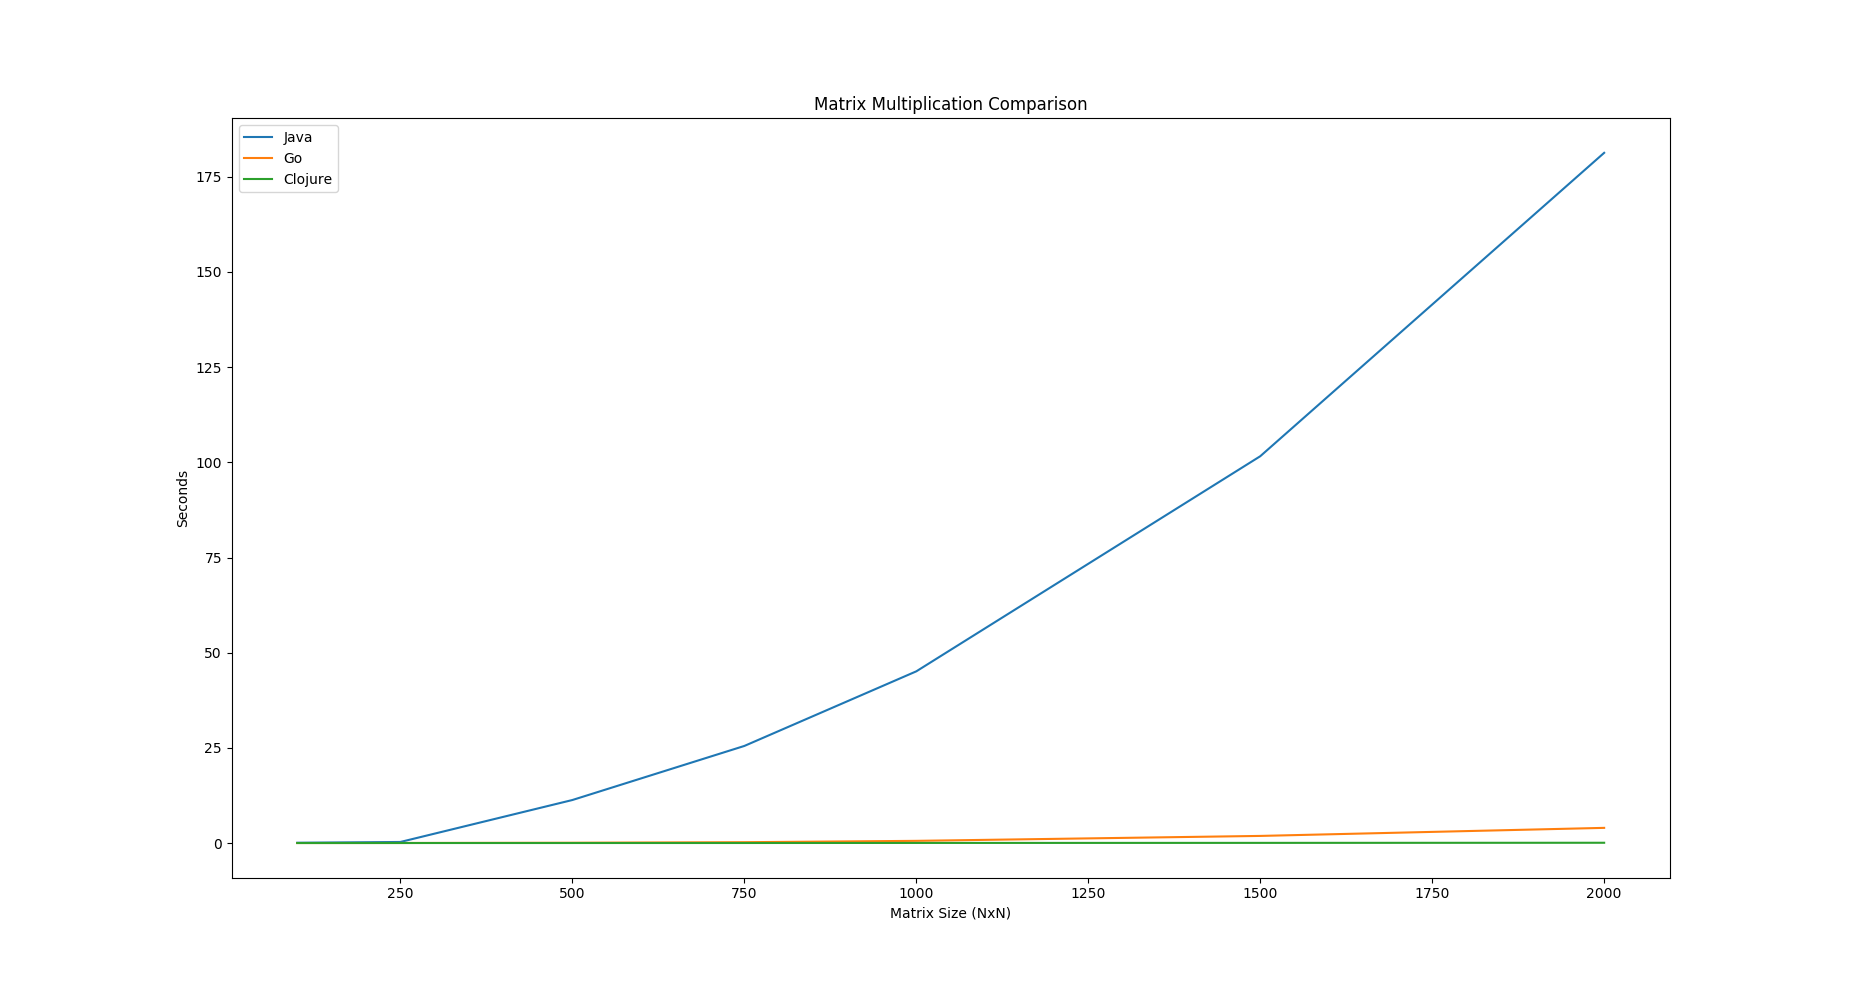
\includegraphics[width=\linewidth,keepaspectratio]{conclusion/comparison.png}

    We would like to do larger comparisons with more hardware, as our brief test could have depending on what hardware each of us used in our implementation and how well they can implement other forms of software such as CUDA or larger frameworks. However, this test does show the improvements when implementing a concurrent language compared to a non-concurrent language, even comparing two languages using the JVM (Java and Clojure).
